\documentclass[tikz,border=2pt]{standalone}
\usepackage{amsmath,amssymb}
\usepackage{pgfplots}
\pgfplotsset{compat=1.18}
\usetikzlibrary{arrows.meta}
\begin{document}
% X ~ Exp(0.01), d = 100: losses below d give Y^L = 0 (probability F_X(d) = 1 - e^{-1} ~ 0.632);
% losses above d give a payment X - d (probability e^{-1} ~ 0.368), whose conditional law Y^P has mean 100.
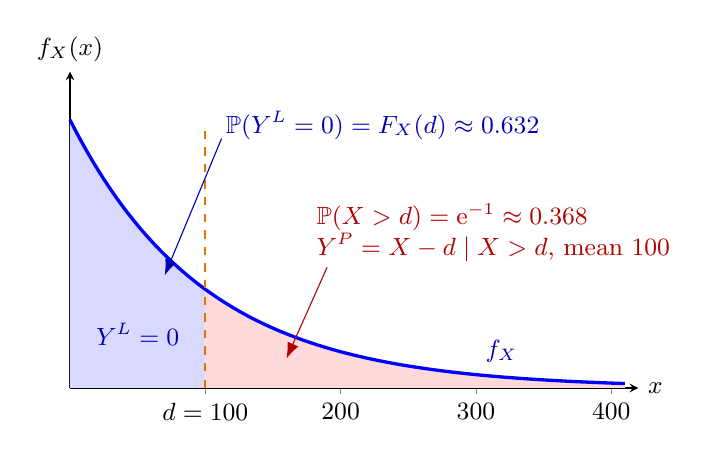
\begin{tikzpicture}[font=\small, >={Latex[length=2mm]}]
  \begin{axis}[
    axis lines=left, xmin=0, xmax=420, ymin=0, ymax=0.0118,
    xtick={100,200,300,400}, xticklabels={$d=100$,$200$,$300$,$400$}, ytick=\empty,
    xlabel={$x$}, ylabel={$f_X(x)$},
    xlabel style={at={(axis description cs:1,0)}, anchor=west},
    ylabel style={rotate=-90, at={(axis description cs:0,1)}, anchor=south},
    samples=120, width=8.8cm, height=5.6cm, clip=false]
    \addplot[fill=blue!15, draw=none, domain=0:100] {0.01*exp(-0.01*x)} \closedcycle;
    \addplot[fill=red!15, draw=none, domain=100:410] {0.01*exp(-0.01*x)} \closedcycle;
    \addplot[blue, very thick, domain=0:410] {0.01*exp(-0.01*x)};
    \draw[orange!90!black, thick, dashed] (axis cs:100,0) -- (axis cs:100,0.0098);
    \node[blue!70!black] at (axis cs:50,0.002) {$Y^L=0$};
    \node[blue!70!black, anchor=west] at (axis cs:108,0.0098) {$\mathbb{P}(Y^L=0)=F_X(d)\approx0.632$};
    \draw[blue!70!black, ->] (axis cs:112,0.0093) -- (axis cs:70,0.0042);
    \node[red!70!black, anchor=west, align=left] at (axis cs:175,0.0058) {$\mathbb{P}(X>d)=\mathrm{e}^{-1}\approx0.368$\\$Y^P=X-d\mid X>d$, mean $100$};
    \draw[red!70!black, ->] (axis cs:190,0.0045) -- (axis cs:160,0.0011);
    \node[blue!70!black, anchor=south west] at (axis cs:300,0.0006) {$f_X$};
  \end{axis}
\end{tikzpicture}
\end{document}
